% Options for packages loaded elsewhere
\PassOptionsToPackage{unicode}{hyperref}
\PassOptionsToPackage{hyphens}{url}
%
\documentclass[
  10pt,
  b5paper,
  oneside]{book}
\usepackage{amsmath,amssymb}
\usepackage{iftex}
\ifPDFTeX
  \usepackage[T1]{fontenc}
  \usepackage[utf8]{inputenc}
  \usepackage{textcomp} % provide euro and other symbols
\else % if luatex or xetex
  \usepackage{unicode-math} % this also loads fontspec
  \defaultfontfeatures{Scale=MatchLowercase}
  \defaultfontfeatures[\rmfamily]{Ligatures=TeX,Scale=1}
\fi
\usepackage{lmodern}
\ifPDFTeX\else
  % xetex/luatex font selection
\fi
% Use upquote if available, for straight quotes in verbatim environments
\IfFileExists{upquote.sty}{\usepackage{upquote}}{}
\IfFileExists{microtype.sty}{% use microtype if available
  \usepackage[]{microtype}
  \UseMicrotypeSet[protrusion]{basicmath} % disable protrusion for tt fonts
}{}
\makeatletter
\@ifundefined{KOMAClassName}{% if non-KOMA class
  \IfFileExists{parskip.sty}{%
    \usepackage{parskip}
  }{% else
    \setlength{\parindent}{0pt}
    \setlength{\parskip}{6pt plus 2pt minus 1pt}}
}{% if KOMA class
  \KOMAoptions{parskip=half}}
\makeatother
\usepackage{xcolor}
\usepackage{longtable,booktabs,array}
\usepackage{calc} % for calculating minipage widths
% Correct order of tables after \paragraph or \subparagraph
\usepackage{etoolbox}
\makeatletter
\patchcmd\longtable{\par}{\if@noskipsec\mbox{}\fi\par}{}{}
\makeatother
% Allow footnotes in longtable head/foot
\IfFileExists{footnotehyper.sty}{\usepackage{footnotehyper}}{\usepackage{footnote}}
\makesavenoteenv{longtable}
\usepackage{graphicx}
\makeatletter
\def\maxwidth{\ifdim\Gin@nat@width>\linewidth\linewidth\else\Gin@nat@width\fi}
\def\maxheight{\ifdim\Gin@nat@height>\textheight\textheight\else\Gin@nat@height\fi}
\makeatother
% Scale images if necessary, so that they will not overflow the page
% margins by default, and it is still possible to overwrite the defaults
% using explicit options in \includegraphics[width, height, ...]{}
\setkeys{Gin}{width=\maxwidth,height=\maxheight,keepaspectratio}
% Set default figure placement to htbp
\makeatletter
\def\fps@figure{htbp}
\makeatother
\setlength{\emergencystretch}{3em} % prevent overfull lines
\providecommand{\tightlist}{%
  \setlength{\itemsep}{0pt}\setlength{\parskip}{0pt}}
\setcounter{secnumdepth}{5}
\usepackage{booktabs}
\usepackage{amsthm}
\makeatletter
\let\stdl@chapter\l@chapter
\renewcommand*{\l@chapter}[2]{%
  \stdl@chapter{\textcolor{astral}{#1}}{\textcolor{astral}{#2}}}

\def\thm@space@setup{%
  \thm@preskip=5cm
  \thm@postskip=\thm@preskip

}
\usepackage{graphicx}
\usepackage{afterpage}

\newcommand\blankpage{%
    \null
    \thispagestyle{empty}%
    \addtocounter{page}{-1}%
    \newpage}

\usepackage{amssymb}
\usepackage{amsmath}
%\pagestyle{plain} % default for report

\usepackage{etoolbox}
\makeatletter
\patchcmd{\@makechapterhead}{50\p@}{-24pt}{}{}
\patchcmd{\@makeschapterhead}{50\p@}{-24pt}{}{}
\makeatother

\makeatother
\usepackage{sectsty}

\definecolor{astral}{RGB}{153, 61, 15}
\allsectionsfont{\sffamily\color{astral}}


\usepackage{fancyhdr}
\usepackage{pdfpages}

\renewcommand{\headrulewidth}{0.5pt}
\renewcommand{\headrule}{\hbox to\headwidth{\color{astral}\leaders\hrule height \headrulewidth\hfill}}


\setlength{\headheight}{5pt}

\fancyhf{}
\fancyhead[EL]{\nouppercase\leftmark}
\fancyhead[OR]{\nouppercase\rightmark}
\fancyhead[ER,OL]{\thepage}

\usepackage{multicol}
\usepackage{hyperref}
\usepackage{longtable}
\usepackage{array}
\usepackage{multirow}
\usepackage{wrapfig}
\usepackage{float}
\usepackage{colortbl}
\usepackage{pdflscape}
\usepackage{tabu}
\usepackage{threeparttable}
\usepackage{adjustbox}
\usepackage{rotating}
\usepackage{tablefootnote}
\usepackage[normalem]{ulem}
% empty pages betwen chapters
\usepackage{emptypage}


\makeatletter
\makeatother

\renewcommand{\listfigurename}{Figures}
\renewcommand{\listtablename}{Tables}

\usepackage[sectionbib]{chapterbib}

%% List of Abbreviations
\usepackage{nomencl}
\makenomenclature
\renewcommand{\nomname}{Acronyms}
%% to update run makeindex on docs folder and move results to / folder
%% see nomencl manual
%% e.g. makeindex SOCMapping.nlo -s nomencl.ist -o SOCMapping.nls

%% index
\usepackage{imakeidx}
\makeindex

\usepackage{xspace}

% no title page
\AtBeginDocument{\let\maketitle\relax}
\hypersetup{
	colorlinks=true,
	linkcolor=astral,
	filecolor=astral,
	urlcolor=astral,
	citecolor=astral
}

\AtBeginDocument{\renewcommand{\chaptername}{Chapter}}
\usepackage{titling}
\usepackage{natbib}
\usepackage{pdfpages}
\usepackage{fancyhdr}
\usepackage{booktabs}
\usepackage{longtable}
\usepackage{subfig}
\usepackage{array}
\usepackage{amsmath}
\usepackage{multirow}
\usepackage{wrapfig}
\usepackage{bookmark}
\usepackage[utf8]{inputenc}
\usepackage{float}
\usepackage{colortbl}
\usepackage{pdflscape}
\usepackage{tabu}
\usepackage{threeparttable}
\usepackage{threeparttablex}
\usepackage[normalem]{ulem}
\usepackage{makecell}
\usepackage{xcolor}
\DeclareUnicodeCharacter{2212}{\textendash}
\usepackage{rotating, graphicx}
\usepackage{listings}
\ifLuaTeX
  \usepackage{selnolig}  % disable illegal ligatures
\fi
\usepackage{bookmark}
\IfFileExists{xurl.sty}{\usepackage{xurl}}{} % add URL line breaks if available
\urlstyle{same}
\hypersetup{
  pdftitle={Integrated Soil Information for decision-making },
  pdfauthor={Angelini, M.E, Rodriguez Lado, L.,de Sousa Mendes, W., Ribeiro, E., Luotto, I.},
  hidelinks,
  pdfcreator={LaTeX via pandoc}}

\title{Integrated Soil Information for decision-making}
\usepackage{etoolbox}
\makeatletter
\providecommand{\subtitle}[1]{% add subtitle to \maketitle
  \apptocmd{\@title}{\par {\large #1 \par}}{}{}
}
\makeatother
\subtitle{From Soil Sampling Design and Spectroscopy to Decision-Making}
\author{Angelini, M.E, Rodriguez Lado, L.,de Sousa Mendes, W., Ribeiro, E., Luotto, I.}
\date{}

\begin{document}
\maketitle

\pagestyle{plain}
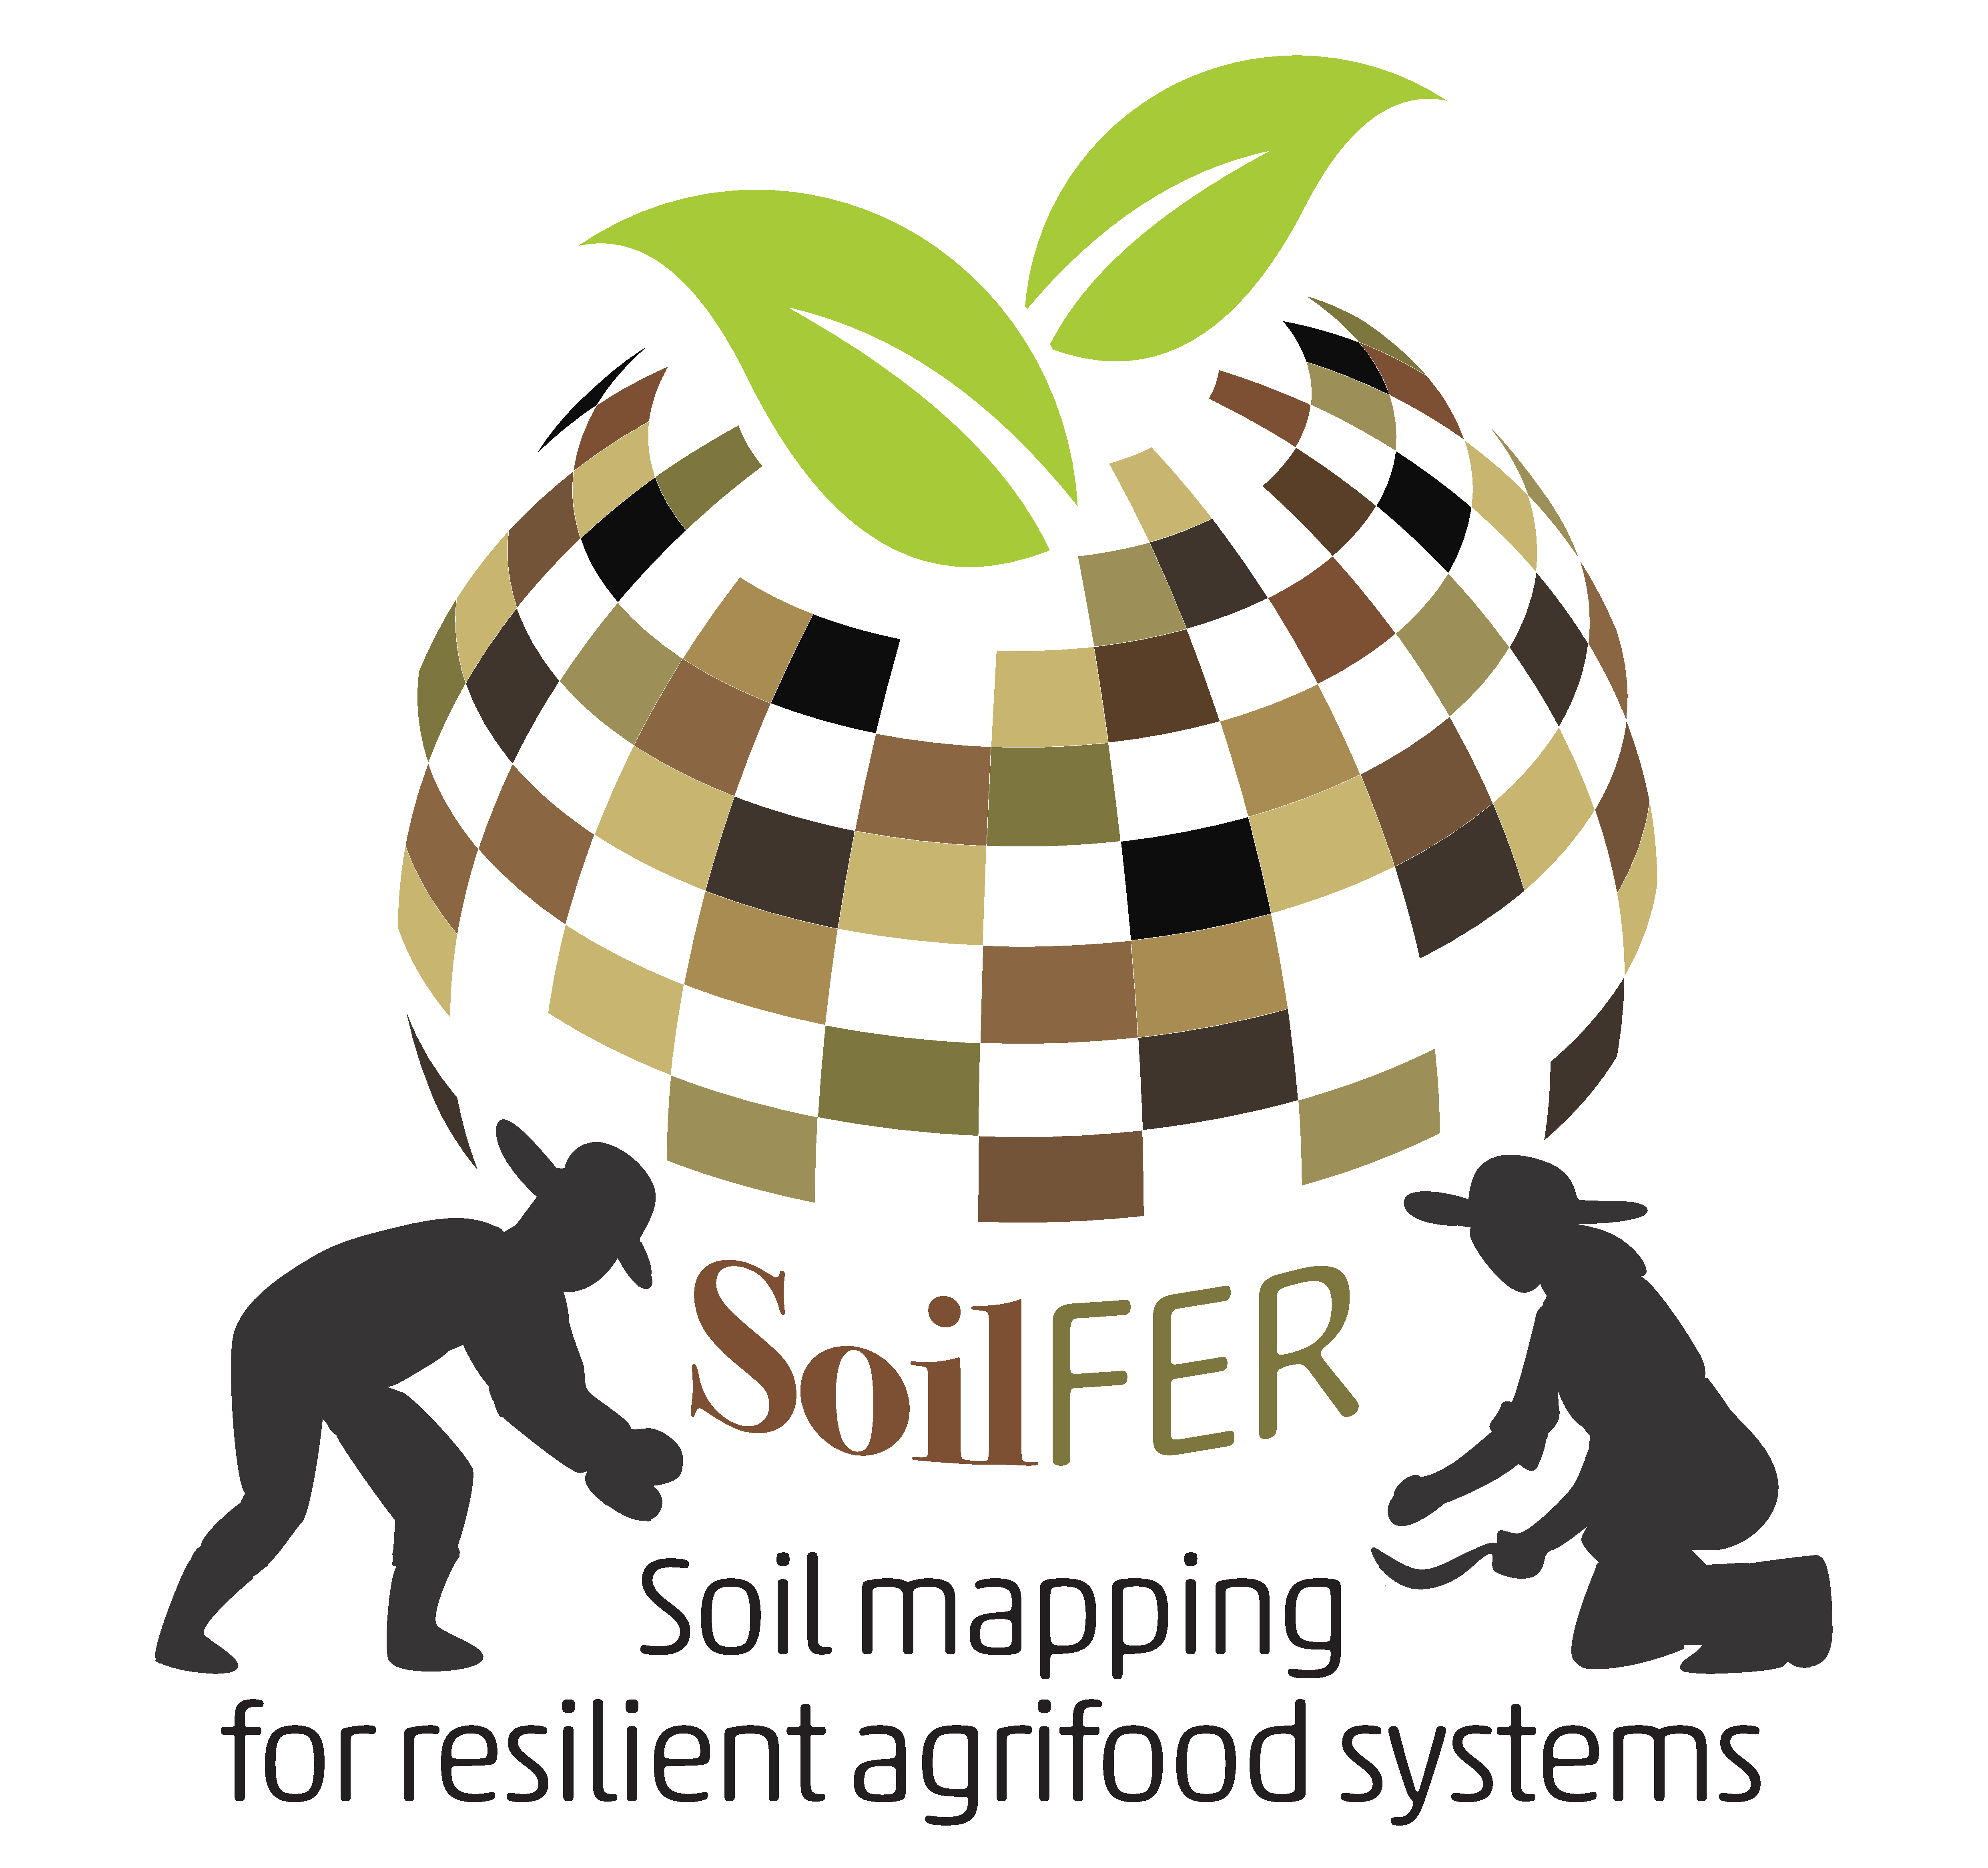
\includepdf{images/frontcover.pdf}
\afterpage{\blankpage}
\thispagestyle{empty}
\begin{titlepage}
    \begin{center}
        \vspace*{4cm}
        \Large

        \textcolor{astral}{\textbf{Global Soil Nutrient and Nutrient Budgets maps (GSNmap) Phase I\\
Technical Manual\\}}
        \vspace{0.5cm}
        \normalsize
        \vfill
        \noindent
        {\color{astral}\rule{\linewidth}{0.5mm} }

        Food and Agriculture Organization of the United Nations\\
	Rome, 2022
    \end{center}
\end{titlepage}
\includepdf{images/CB9015EN_Copyright Disclaimer_v2.pdf}


\frontmatter
\addtocontents{toc}{\protect\hypersetup{hidelinks}}   
\addtocontents{lof}{\protect\hypersetup{hidelinks}}
\addtocontents{lot}{\protect\hypersetup{hidelinks}}
\addtocontents{lot}{\protect\hypersetup{hidelinks}}
\addtocontents{lot}{\protect\hypersetup{hidelinks}}
\tableofcontents
\listoffigures
\listoftables
\nopagebreak[5]

\begin{figure}
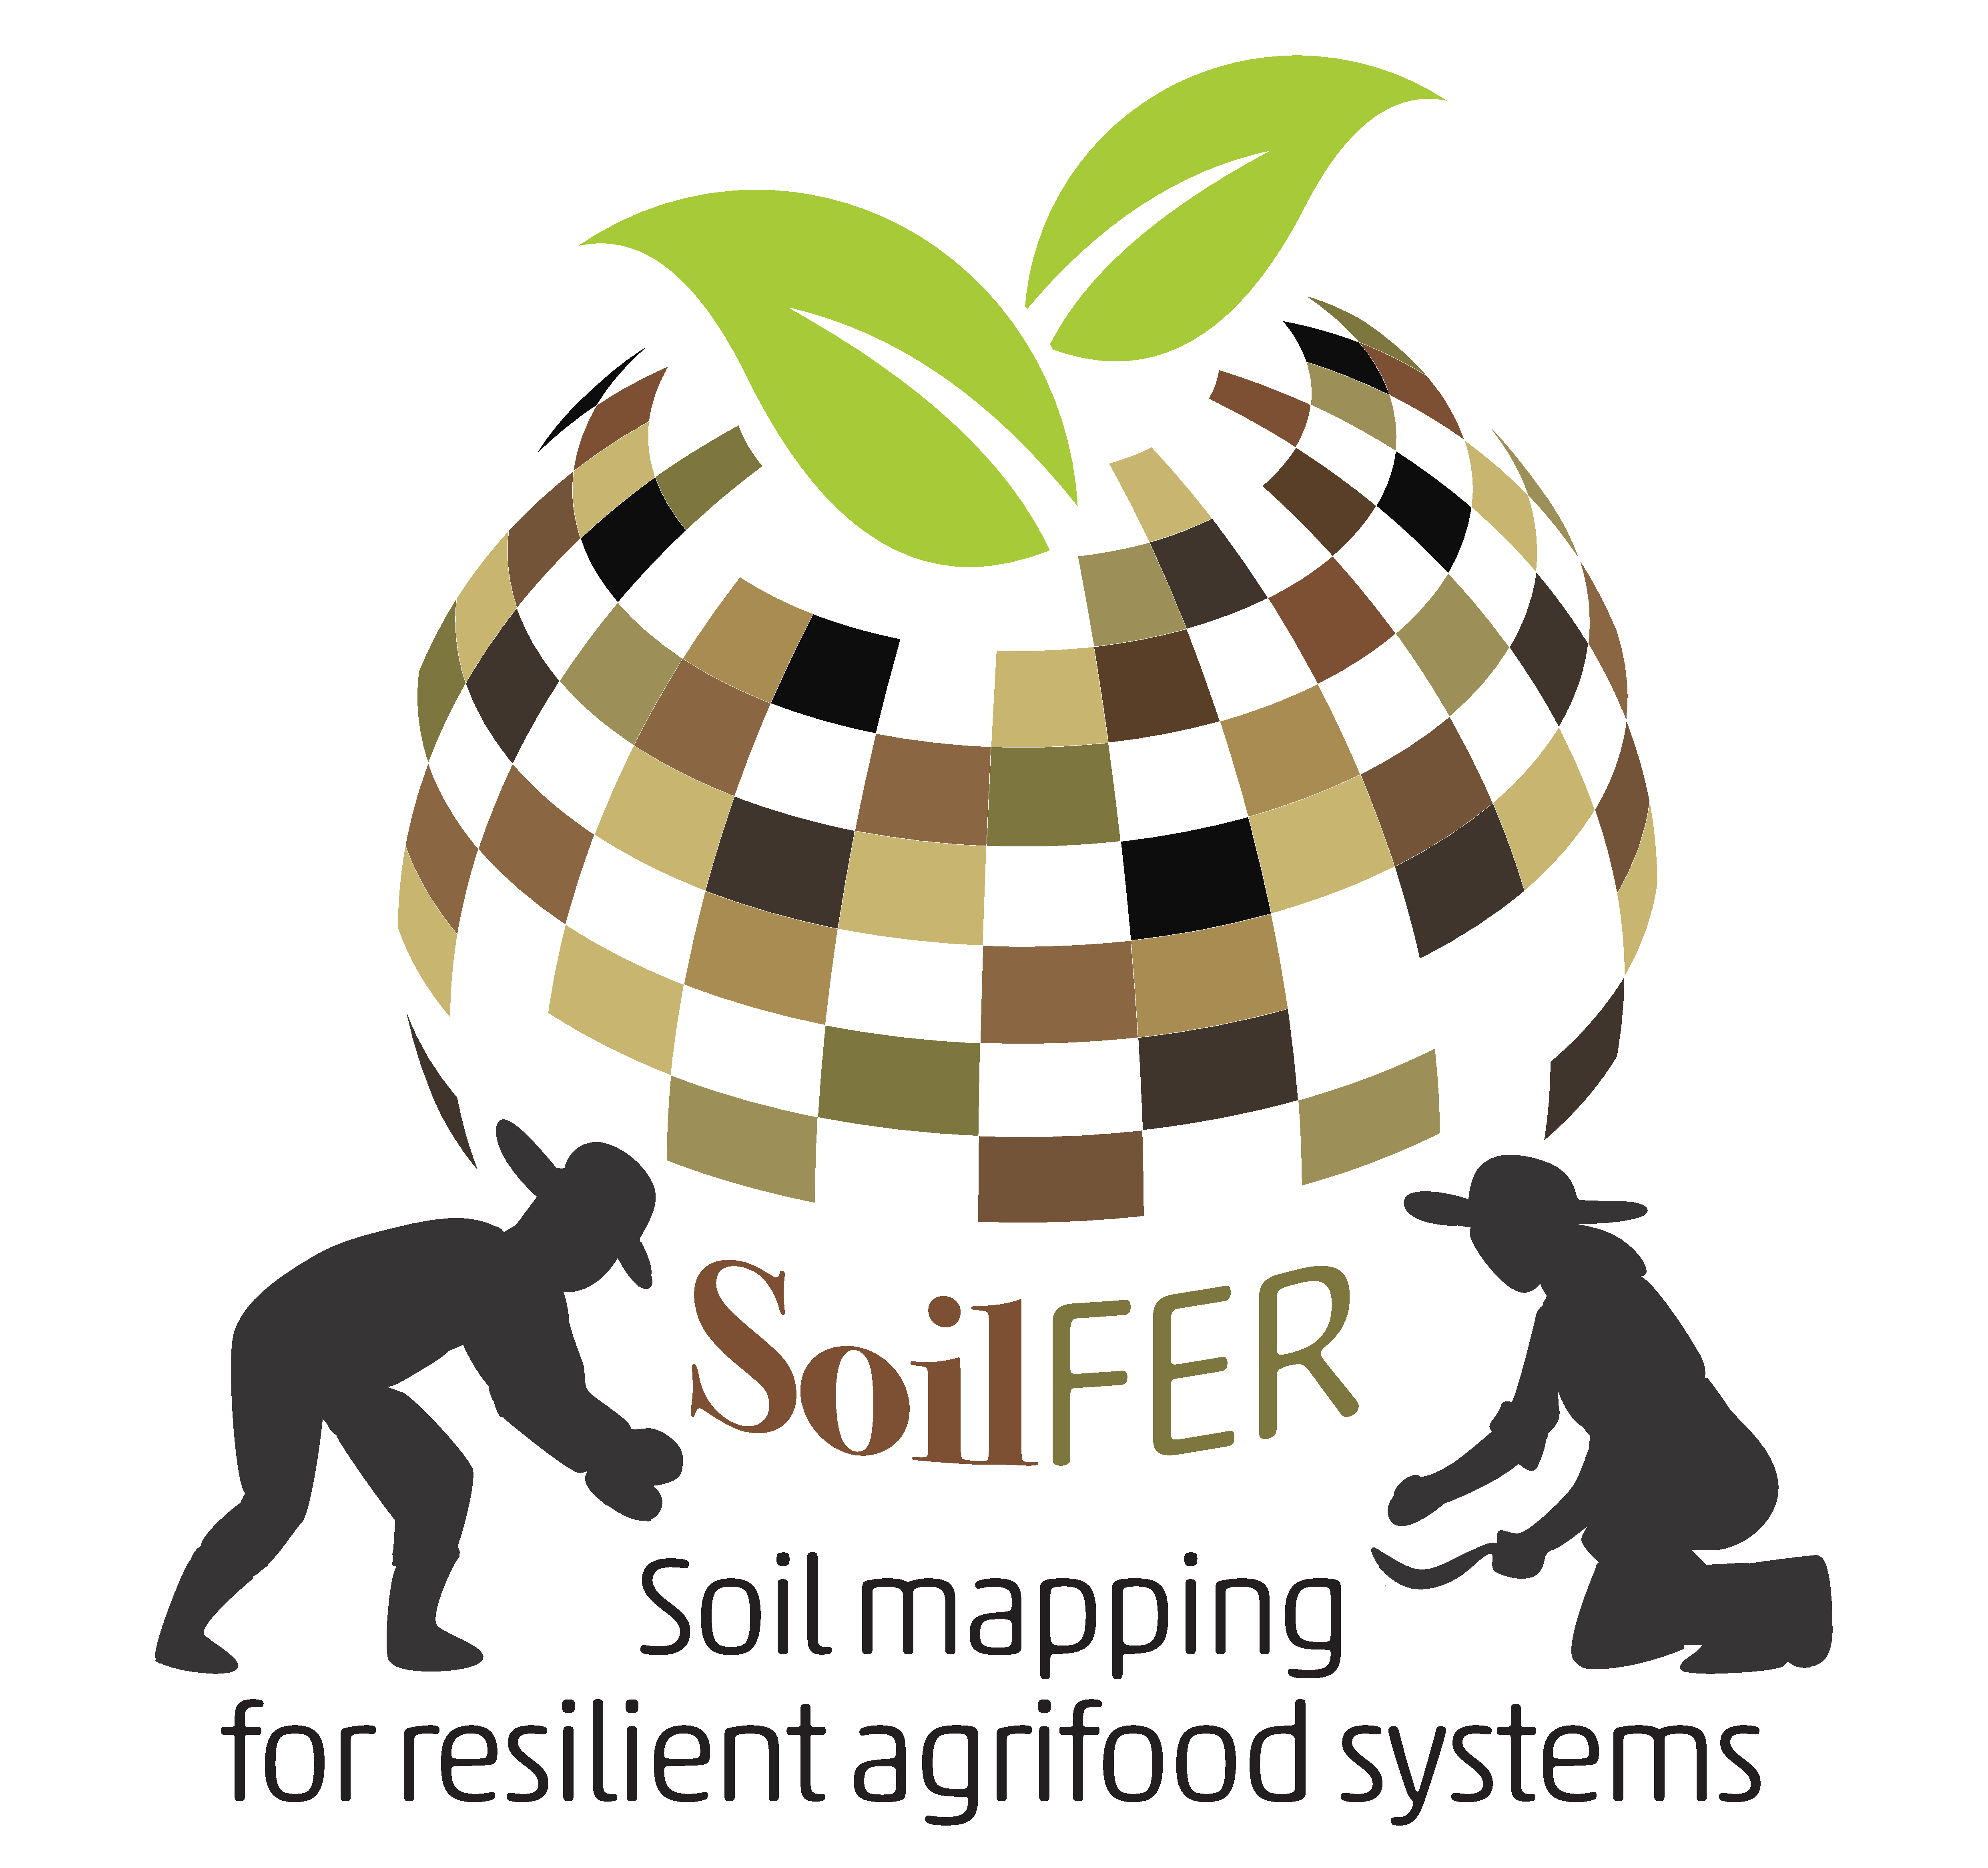
\includegraphics[width=41.67in]{images/frontcover} \end{figure}

\chapter*{Licence}\label{licence}
\addcontentsline{toc}{chapter}{Licence}

The Technical Manual is made available under the Creative Commons Attribution-NonCommercial-ShareAlike 3.0 IGO licence

\href{https://creativecommons.org/licenses/by-nc-sa/3.0/igo/legalcode}{CC BY-NC-SA 3.0 IGO}.

\chapter*{Abbreviations and acronyms}\label{abbreviations-and-acronyms}
\addcontentsline{toc}{chapter}{Abbreviations and acronyms}

\begin{description}
\item[BD]
Bulk density
\item[CEC]
Cation exchange capacity
\item[CRAN]
Comprehensive R archive network
\item[DSM]
Digital soil mapping
\item[GEE]
Google Earth Engine
\item[GSP]
Global Soil Partnership
\item[INSII]
International Network of Soil Information Institutions
\item[ITPS]
Intergovernmental Technical Panel on Soils
\item[ME]
Mean error
\item[MAE]
Mean absolute error
\item[MEC]
Modelling efficiency coefficient
\item[NDVI]
Normalized difference in vegetation index
\item[QA/QC]
Quality assurance/quality check
\item[RMSE]
Root mean squared error
\item[SOC]
Soil organic carbon
\item[SOM]
Soil organic matter
\end{description}

\chapter*{Contributors and reviewers}\label{contributors-and-reviewers}
\addcontentsline{toc}{chapter}{Contributors and reviewers}

\chapter{Presentation and basics}\label{presentation-and-basics}

Placeholder

\section{How to use this book}\label{how-to-use-this-book}

\section{Training material}\label{training-material}

\section{Setting up the software environment}\label{setting-up-the-software-environment}

\subsection{Digital Soil Mapping}\label{digital-soil-mapping}

\subsection{Main concepts: SCORPAN model}\label{main-concepts-scorpan-model}

\chapter{Sampling design for soil surveys}\label{sampling-design-for-soil-surveys}

Placeholder

\section{Selection of the sampling methodology}\label{selection-methods}

\section{Inference Methods}\label{inference-methods}

\section{Purpose of Sampling}\label{sampling-purpose}

\section{Sampling Design Types}\label{design-types}

\subsection{Example: Soils4Africa Sampling Design}\label{soils4africa-example}

\section{Soil Properties}\label{soil-properties}

\section{Environmental Covariates}\label{env-covariates}

\section{Understanding the Methodology}\label{methodology}

\subsection{PSU Selection Process}\label{psu-selection-process}

\subsection{SSU and TSU Selection Process}\label{ssu-tsu-selection}

\subsection{Site Identification System}\label{site-id}

\section{Setting Up the Environment}\label{setup}

\subsection{Install Required Libraries}\label{install-libraries}

\section{Define Variables and Parameters}\label{define-parameters}

\subsection{Country ISO Code}\label{country-iso-code}

\subsection{Land Use Type}\label{land-use-type}

\subsection{File Paths}\label{file-paths}

\subsection{Coordinate Reference System}\label{coordinate-reference-system}

\subsection{Sample Size Calculation}\label{sample-size-calculation}

\subsection{Sampling Unit Definitions}\label{sampling-unit-definitions}

\subsection{Algorithm Parameters}\label{algorithm-parameters}

\section{Custom Functions}\label{custom-functions}

\subsection{Covariate Space Coverage Function (CSIS)}\label{covariate-space-coverage-function-csis}

\subsection{TSU Generation Function}\label{tsu-generation-function}

\section{Load Country Boundaries and Legacy Data}\label{load-boundaries}

\subsection{Visualize Boundaries and Legacy Data}\label{visualize-boundaries-and-legacy-data}

\section{Load Environmental Covariates for PSUs}\label{load-covariates-psu}

\subsection{Optional Auxiliary Data}\label{optional-auxiliary-data}

\subsection{Load and Process Auxiliary Data}\label{load-and-process-auxiliary-data}

\subsection{Load Main Environmental Covariates}\label{load-main-environmental-covariates}

\subsection{Load and Process Soil Climate Data (Newhall)}\label{load-and-process-soil-climate-data-newhall}

\subsection{Convert Categorical Variables to Dummy Variables}\label{convert-categorical-variables-to-dummy-variables}

\subsection{Merge All Covariate Layers}\label{merge-all-covariate-layers}

\subsection{Crop and Save Covariates}\label{crop-and-save-covariates}

\section{Principal Component Analysis (PCA)}\label{pca}

\section{Organize the Sampling Universe}\label{sampling-universe}

\subsection{Load and Process Land Use Data}\label{load-and-process-land-use-data}

\subsection{Exclude Protected Areas}\label{exclude-protected-areas}

\subsection{Restrict to Accessible Slopes}\label{restrict-to-accessible-slopes}

\subsection{Aggregate to 100m Resolution}\label{aggregate-to-100m-resolution}

\subsection{Save Processed Land Use}\label{save-processed-land-use}

\subsection{Filter Legacy Data}\label{filter-legacy-data}

\section{Create Primary Sampling Units (PSU Grid)}\label{create-psu-grid}

\subsection{Generate 2km × 2km Grid}\label{generate-2km-2km-grid}

\subsection{Trim to Country Boundaries}\label{trim-to-country-boundaries}

\subsection{Save PSU Grid}\label{save-psu-grid}

\section{Select PSUs with Sufficient Land Use Coverage}\label{select-psus}

\subsection{Calculate Land Use Percentage}\label{calculate-land-use-percentage}

\subsection{Filter PSUs}\label{filter-psus}

\section{Rasterize PSUs for Covariate Space Coverage}\label{rasterize-psus}

\section{Compute Optimal Sample Size}\label{optimal-sample-size}

\subsection{Run Optimization}\label{run-optimization}

\subsection{Extract Optimal Sample Size}\label{extract-optimal-sample-size}

\section{Covariate Space Coverage - Computing PSUs}\label{csc-computing}

\subsection{Prepare Function Parameters}\label{prepare-function-parameters}

\subsection{Perform K-means Clustering}\label{perform-k-means-clustering}

\subsection{Assign Clusters and Calculate Distances}\label{assign-clusters-and-calculate-distances}

\subsection{Extract Selected PSUs}\label{extract-selected-psus}

\subsection{Visualize in Covariate Space}\label{visualize-in-covariate-space}

\section{Compute SSUs and TSUs}\label{compute-ssu-tsu}

\subsection{Load High-Resolution Covariates}\label{load-high-resolution-covariates}

\subsection{Process Each PSU}\label{process-each-psu}

\subsection{Combine SSUs and TSUs}\label{combine-ssus-and-tsus}

\section{Export Sampling Units}\label{export-units}

\subsection{Create Cluster Raster}\label{create-cluster-raster}

\subsection{Join Cluster Info to TSUs}\label{join-cluster-info-to-tsus}

\subsection{Create Site IDs}\label{create-site-ids}

\subsection{Export Shapefiles}\label{export-shapefiles}

\section{Compute Alternative PSUs}\label{alternative-psus}

\section{Assign Country-Wide Unique IDs}\label{assign-unique-ids}

\section{Export Unified Datasets}\label{export-unified}

\section{Summary Statistics}\label{summary-stats}

\section{Create Distribution Maps}\label{distribution-maps}

\section{GPS Device Preparation}\label{gps-prep}

\subsection{Export to GPX Format}\label{export-to-gpx-format}

\subsection{Load onto GPS Device}\label{load-onto-gps-device}

\section{Sampling Procedure}\label{sampling-procedure}

\section{Data Recording}\label{data-recording}

\section{Quality Control}\label{qc}

\section*{Appendix A: Software and Data Sources}\label{appendix-a-software-and-data-sources}
\addcontentsline{toc}{section}{Appendix A: Software and Data Sources}

\subsection{Software Requirements}\label{software-requirements}

\subsection{Data Sources}\label{data-sources}

\section*{Appendix B: Troubleshooting Common Issues}\label{appendix-b-troubleshooting-common-issues}
\addcontentsline{toc}{section}{Appendix B: Troubleshooting Common Issues}

\subsection{Memory Issues}\label{memory-issues}

\subsection{CRS Misalignment}\label{crs-misalignment}

\subsection{Empty Geometry}\label{empty-geometry}

\section*{Appendix C: Acronyms and Abbreviations}\label{appendix-c-acronyms-and-abbreviations}
\addcontentsline{toc}{section}{Appendix C: Acronyms and Abbreviations}

\chapter{TBD}\label{tbd}

\chapter{Soil Data Preparation}\label{soil-data-preparation}

\section{Introduction}\label{introduction}

\section{Data cleaning}\label{data-cleaning}

\section{Soil Data Harmonization}\label{soil-data-harmonization}

\section{Concepts on digital exchange of soil-related data (ISO 28258)}\label{concepts-on-digital-exchange-of-soil-related-data-iso-28258}

\section{Plot data}\label{plot-data}

\section{Profile data}\label{profile-data}

\section{Element data}\label{element-data}

\section{Specimen data}\label{specimen-data}

\section{Definition of laboratory procedures}\label{definition-of-laboratory-procedures}

\section{Data transformation}\label{data-transformation}

\section{Organizing soil data according to the GloSIS database}\label{organizing-soil-data-according-to-the-glosis-database}

\section{Tools for harmonization of soil databases within GloSIS}\label{tools-for-harmonization-of-soil-databases-within-glosis}

\chapter{Digital soil mapping and modeling}\label{digital-soil-mapping-and-modeling}

\chapter{Soil Data Sharing}\label{soil-data-sharing}

\section{Data sharing and export formats}\label{data-sharing-and-export-formats}

\section{Metadata}\label{metadata}

\section{Web Services}\label{web-services}

\chapter*{References}\label{references}
\addcontentsline{toc}{chapter}{References}

%\printindex
\includepdf{images/backcover.pdf}

\end{document}
